
\documentclass[preprint,12pt]{elsarticle}

\usepackage[spanish]{babel}
\usepackage{amssymb}
\usepackage{graphicx}
\usepackage{lineno}
\usepackage[utf8]{inputenc}
\usepackage{url}
\usepackage{natbib}

\begin{document}
	
	\begin{frontmatter}

		\title{\huge  Comparativa de Cuadro de Mando Integral (BSC) y Modelo de Negocio Canvas (BMC) }
		\author{Robles Flores, Anthony Richard	                (2016056192)}
		\author{Estrella Palacios, Katherine Lizbeth			(2015050948)}
		\author{Sosa Bedoya, Sharon Fiorela				(2016054460)}
		\author{Torres Beltran , Johanna Andrea			(2020067849)}
		\address{Tacna, Perú}
		


%%INICIO abstract
\begin{abstract}

\end{abstract}
%%FIN abstract


\end{frontmatter}

%%INICIO Resumen
\section{Resumen}

%%FIN Resumen


%%INICIO Introducción
\section{Introducción}


%%FIN Introducción


%%INICIO Marco Teórico
\section{Marco Teórico}

%%----------------------------------------------------------------------------------------------------------------------------------------------------------
	\subsection{\textbf{Cuadro de Mando Integral (BSC)}}
	
xxxxxxxxxxxxxxxxxxxxxxxxxxxxxxxxxxxxxxxxxxxxxxxxxxxxxxxxxxxxxxxxxxxxxxxxxxxxxxxxxxxxxxxxxxx\cite{referenciarobles1}

\subsubsection{\textbf{Subtitulo 1}}

	\begin{itemize}
	\item a
	\item b
	\item c
	\end{itemize}



\subsubsection{\textbf{Subtitulo 2}}

	\begin{itemize}
	\item a
	\item b
	\item c
	\end{itemize}

%%----------------------------------------------------------------------------------------------------------------------------------------------------------

	\subsection{\textbf{Modelo de Negocio Canvas (BMC) }}
	
xxxxxxxxxxxxxxxxxxxxxxxxxxxxxxxxxxxxxxxxxxxxxxxxxxxxxxxxxxxxxxxxxxxxxxxxxxxxxxxxxxxxxxxxxxxxxxxxxxxxxxxxxxxx

	\subsubsection{\textbf{Subtitulo 1}}
	\begin{itemize}
	\item{\textbf{1. Punto1: }}XXXXXXXXXXXXX
	\item {\textbf{2. Punto2: }}XXXXXXXXXXXX
	\item {\textbf{3. Punto3: }}XXXXXXXXXXXX
	\end{itemize}

	\subsubsection{\textbf{Subtitulo 2}}

	\begin{itemize}
	\item a
	\item b
	\item c
	\end{itemize}

	\subsubsection{\textbf{Subtitulo 3}}

	\begin{figure}[htb]
		\begin{center}
			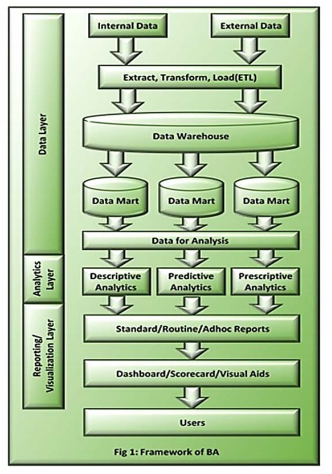
\includegraphics[height=9cm]{./IMAGENES/BAFramework} 
			\caption{Framework de BA}
		\end{center}
	\end{figure}


%%FIN Marco Teórico
%%----------------------------------------------------------------------------------------------------------------------------------------------------------


%COMPRACION

\section{Comparación entre Cuadro de Mando Integral (BSC) y Modelo de Negocio Canvas (BMC)}
A continuación se muestra la comparación entre Cuadro de Mando Integral (BSC) y Modelo de Negocio Canvas (BMC)
	
	\begin{itemize}

	\item{\textbf{1.}} XXXXXXXXXXXXXXXXXXXX
	\item{\textbf{2.}} XXXXXXXXXXXXXXXXXXXX
	\item{\textbf{3.}} XXXXXXXXXXXXXXXXXXXX
	\item{\textbf{4.}} XXXXXXXXXXXXXXXXXXXX
	\item{\textbf{5.}} XXXXXXXXXXXXXXXXXXXX
	\item{\textbf{6.}} XXXXXXXXXXXXXXXXXXXX
	\item{\textbf{7.}} XXXXXXXXXXXXXXXXXXXX
	\end{itemize}

%%----------------------------------------------------------------------------------------------------------------------------------------------------------

%CONCLUSIONES
\section{Conclusiones}

%%****
	\begin{itemize}
		\item XXXXXXXXXXXXXXXXXXXX
		\item XXXXXXXXXXXXXXXXXXXX
		\item XXXXXXXXXXXXXXXXXXXX
	\end{itemize}

%%----------------------------------------------------------------------------------------------------------------------------------------------------------

%RECOMENDACIONES
\section{Recomendaciones}	

	\begin{itemize}
		\item XXXXXXXXXXXXXXXXXXXX
		\item XXXXXXXXXXXXXXXXXXXX
		\item XXXXXXXXXXXXXXXXXXXX
	\end{itemize}


%%----------------------------------------------------------------------------------------------------------------------------------------------------------

	
	\newpage
	\bibliographystyle{apalike}
	\bibliography{BIBLIOGRAFIA}	



\end{document}

